\chapter{Software Requirement Specifications}
\section{Introduction}
\subsection{Purpose}
To find the relevant content from the huge number of PDF files present on Hadoop Distributed File System. \\

\subsection{Intended Audience}
\subsubsection{Stakeholders}
Stakeholders in a  business organization include creditors, customers, directors, employees, government, owners, suppliers, unions and the community from which the business draw its resources. There are many stakeholders in a single project of different levels.\\
In our project there are mainly 2 stakeholders namely:\\

\begin{enumerate}
\item Hadoop User : The hadoop user can use this API to implement content based search in any particular operation.
\item Application User : Application User is an person in the system who will use the hadoop to perform content based search and retrieval operations on pdfs in HDFS.
\end{enumerate}

\subsection{Scope}
\paragraph{} This system shall retrieve the required contents of files which are in an unstructured format containing huge amount of Data like e-books in a digital library where the number of books are present in thousands. The scope here is initially limited to PDF files which may be expanded to other unstructured formats like ePUB, mobi.
\paragraph{} The input is provided to the system API in the form of search query which will be firstly filtered to find the important expression as a query to the API which will return the important content to the user in the form of paragraph or text highlighted using the power of distributed computing.
\paragraph{} The particular page or the Entire book itself can be downloaded by the Library users if the content is satisfied else the search continues for finding relevant content.

\subsection{Implementation constraints}
\paragraph{} Along with Hadoop Implementation an add-on in the form of JAR library shall be included by the developer using this system which will provide API for high speed retrieval of relevant content.  This API will basically assume to be a multinode cluster installed in the deployed environment.
\paragraph{} The data store API for content based retrieval shall be purely implemented in JAVA which on future shall be implemented for Python and C++ as well.
\paragraph{} There will be basic tokenization of input string and numerous possibilities will be searched distributively on various nodes using the map reduce.
\paragraph{} The final result shall be obtained by the master node and will be passed on to the client application for viewing the results.
\paragraph{} On a future note, Apache spark shall be used to implement this system for speed incremental purposes in case of limitations in the speed of map reduce algorithm.


\subsection{Assumptions And Dependencies}
\begin{itemize}
\item Any Open Source Linux Distribution.(Ubuntu Server version 14.04.2 Preferred)
\item OPENSSH installed on each machine with public key of each node in authorized\_keys directory along with the localhost.
\item JDK Version 1.7 or above
\item JAVA\_HOME to be appended in the \$PATH environment variable
\item Hostname to be initialized for each node in the /etc/hosts file having a masternode (namenode), secondary namenode and various slave nodes to be added.
\item \$HADOOP\_HOME environment variable path to added in the ~/.bashrc 
\item Following Files to be configured in \$HADOOP\_HOME/etc/hadoop directory

	\begin{enumerate}
	\item core-site.xml
	\item hadoop-env.sh
	\item yarn-site.xml
	\item mapred-site.xml
	\item master
	\item slave
	\end{enumerate}

\item Master node with Ubuntu Workstation version preferred for supporting Eclipse IDE with Hadoop plugin for development and Server having Ubuntu Server version Preferred.
\end{itemize}


\section{System Features}

\subsection{Add a document to the system}
User simply needs to upload a file on the system. The system
Should create an appropriate metadata from it and store it in the index.

\subsection{Indexing the Data/Creating a metadata}
Whenever the user uploads a file or updates, system should read the file create a metadata for a new file by adding the title as an index and for an update it should check the changes and update the title of the same.

\subsection{Entering the keyword/s}
User will have to enter keyword/s in the search box in order to obtain desired results, system should take the keyword input and validate it and search the metadata.

\subsection{Validating a keyword}
User may make a mistake like some use of unnecessary words or some spelling mistake while entering a keyword, system should validate that keyword and find the most relevant keyword from the given input. For this operation system should use a validating keyword algorithm.

\subsection{Ranking the documents}
System should use a ranking algorithm to rank the documents stored in it. It may contain more page hits and other factors required for ranking.
Filtering of files before searching for content.

\subsection{Downloading the content}
When a user finds the necessary content, system should ask him how he/she wants the content to be retrieved, whether the complete document or that same page or some more pages before and after that page.
Page by page content search on filtered documents

\section{External Interface Requirements}
\subsection{Hardware Interface}
\begin{itemize}	
\item Memory require for Hadoop installation and HBase and Map Reduce components.
\item API requires minimum 100 MB space as it contains core components for content based retrieval
\item 4 GB Primary Memory / RAM
\item Intel i3/i5/i7 64bit or AMD Processors
\item SSH Authentication to communicate with Namenode and Datanodes
\end{itemize}

\subsection{Software Interface}
\begin{itemize}
\item Any Open Source Linux Distribution.(Ubuntu Server version 14.04.2 Preferred)
\item OPENSSH installed on each machine with public key of each node in authorized\_keys directory along with the localhost.
\item JDK Version 1.7 or above
\item JAVA\_HOME to be appended in the \$PATH environment variable
\item Hostname to be initialized for each node in the /etc/hosts file having a masternode (namenode), secondary namenode and various slave nodes to be added.
\item \$HADOOP\_HOME environment variable path to added in the ~/.bashrc 
\item Following Files to be configured in \$HADOOP\_HOME/etc/hadoop directory
\end{itemize}

\section{Non-functional Requirements}
\subsection{Performance Requirements}
Memory Requirements:
\begin{itemize}	
\item Memory require for Hadoop installation and HBase and Map Reduce components.
\item API requires minimum 100 MB space as it contains core components for content based retrieval
\item 4 GB Primary Memory / RAM
\end{itemize}

Speed Requirements:
\begin{itemize}
\item Intel i3/i5/i7 64bit or AMD Processors
\end{itemize}

\subsection{Security Requirements}
\begin{itemize}
\item SSH Authentication to communicate with Namenode and Datanodes
\end{itemize}

\subsection{Software Quality Attributes}

Software Quality can be defined as “the conformance to explicitly stated functional and performance requirements, explicitly documented development standards, and implicit characteristics that are expected of all professionally developed software”.\\
	
\subsection{Software Quality Attributes are}

\begin{enumerate}
\item \textbf{Functionality} \\
This is an ability by which the software satisfies the needs of the software denoted by suitability, accuracy, interoperability, compliance and security.

\item \textbf{Reliability} \\
Due to wired connectivity, reliability can be guaranteed.

\item \textbf{Availability} \\
The system should be available during their respected hours.

\item \textbf{Usability} \\
This ability indicates that the usefulness of the software.

\item \textbf{Efficiency} \\
This indicates the measure of computing resources and time required by the program to perform.

\item \textbf{Maintainability} \\
The ability required to locate or fix bugs in software. There should be facility to add or delete or update documents.

\item \textbf{Portability} \\
The software works properly even if the environment gets changed (i.e. change in hardware or software).

\item \textbf{Reusability} \\
With new versions of Hadoop this API can be improved using new features of Hadoop
\end{enumerate}

\section{Analysis Models}

\subsection{Data Flow Diagram}

\begin{figure}[h]
\begin{center}
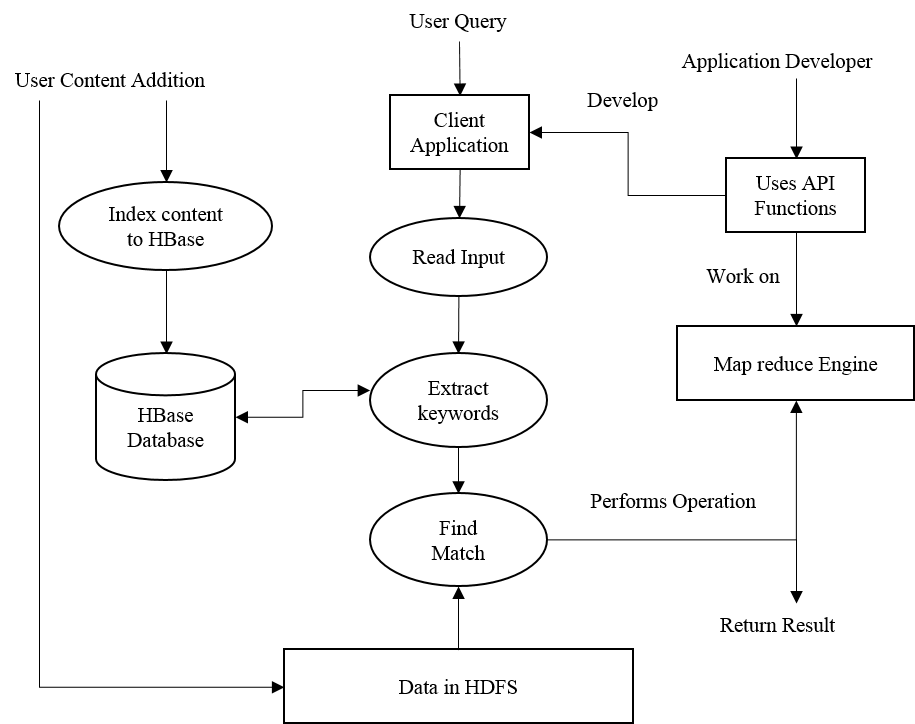
\includegraphics{data_flow}
\end{center}
\caption{Data Flow Diagram}
\end{figure}

\subsection{Class Diagram}

\begin{figure}[h]
\begin{center}
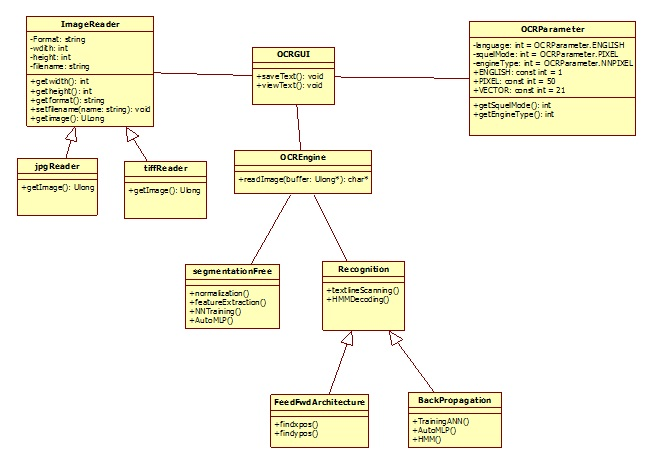
\includegraphics[scale=1]{class.jpg}
\end{center}
\caption{Class Diagram}
\end{figure}

\section{System Implementation Plan}
\begin{table}[!htbp]
\begin{center}
\def\arraystretch{1.5}
  \begin{tabular}{| c | c | c | c |}
       \hline

	\textbf{Activity} & \textbf{Weeks to Spend} & \textbf{Deliverables} & \textbf{Priority}\\ \hline
	Analysis of Existing System & 2 weeks & - & Normal \\ \hline
	Requirement Gathering & 2 weeks & Requirements & Normal \\ \hline 
	Literature Survey & 3 Week & - & Normal \\ \hline
	Designing and Planning & 5 weeks & Modules & High \\ \hline
	Implementation & 10 weeks & API & High \\ \hline
	Testing & 3 weeks & Test Report & High \\ \hline
	Documentation & 4 week & Project Report & Normal \\ \hline
\end{tabular}
 \caption { Plan of Project Execution }
 \label{tab:hreq}
\end{center}

\end{table}